% L11a lecture companion. Notebook hashes and coverage are recorded in README.md.
% Style files and Cornell seal are copied unchanged from the L10c deck (identical
% to L10a, L9c, and L9a, which match the approved L6a deck). The three figures
% are converted from the notebook SVGs in ../figs by `make figures`.
%
% Notation follows the lecture: the Markov model M = (S, P), states s_1, ..., s_N,
% the state X_n at time step n, one-step probabilities p_ij, row distributions
% pi_n, the stationary distribution \bar{pi}, the tolerance epsilon, the
% iteration limit T, and the iteration counter t.
\documentclass[aspectratio=169,11pt]{beamer}
\usepackage{vnslides}
\renewcommand{\vnlecturecode}{L11a}
\newcommand{\lecturelink}{https://github.com/varnerlab/CHEME-5800-CourseRepository-Fall-2026/blob/main/weeks/week-11/L11a/CHEME-5800-L11a-Lecture-MarkovModels-Fall-2026.ipynb}
\newcommand{\examplelink}{https://github.com/varnerlab/CHEME-5800-CourseRepository-Fall-2026/blob/main/weeks/week-11/L11a/CHEME-5800-L11a-Example-MarkovModels-Fall-2026.ipynb}
\newcommand{\lablink}{https://github.com/varnerlab/CHEME-5800-CourseRepository-Fall-2026/blob/main/weeks/week-11/L11b/CHEME-5800-L11b-Lab-MarkovWordGenerator-Fall-2026.ipynb}
\newcommand{\lecturesource}[1]{\note{[Sources]\par
  \href{\lecturelink}{L11a lecture: Foundations of Markov Models and Markov Chains.}\par
  #1\par[/Sources]}}
\newcommand{\Sset}{\mathcal S}
\newcommand{\Pm}{\mathbf P}
\newcommand{\pib}{\bar{\pi}}

\title{\texorpdfstring{{\vnheavy L11a}}{L11a}: Markov Models and Markov Chains}
\subtitle{\texorpdfstring{The Markov property, the transition matrix, and the stationary distribution\\[3pt]CHEME 5800 Cornell University}{The Markov property, the transition matrix, and the stationary distribution; CHEME 5800 Cornell University}}
\author{Copyright Jeffrey Varner 2026. All Rights Reserved}

\begin{document}
\special{pdf:minorversion 7}
\vntitlepage

\begin{frame}{Objectives for Today}
  How do we model a random system whose next state depends only on where it
  is now?

  \vspace{0.4em}
  {\large\textbf{\ink{Today's concepts}}}
  \vspace{0.2em}
  \begin{itemize}\setlength{\itemsep}{0.4em}
    \item \hilite{Describe the Markov property}: the probability of the next
      state depends only on the present state, which makes random systems much
      easier to model and analyze.
    \item \hilite{Build a transition matrix}: hold the probability of moving
      from each state to every state in one time step, and state the properties
      every row must satisfy.
    \item \hilite{Compute the stationary distribution}: find the distribution
      that the transition matrix leaves unchanged, using power iteration.
  \end{itemize}
  \slidenote{Lecture:}{\href{\lecturelink}{Foundations of Markov Models and Markov Chains}}
  \lecturesource{Introduction and three Learning Objectives.}
\end{frame}

\begin{frame}{Lecture and Example}
  \textbf{\ink{Lecture:}}
  \href{\lecturelink}{Foundations of Markov Models and Markov Chains}

  In this lecture, we define the Markov property, collect the one-step
  transition probabilities in a matrix, and compute the stationary distribution
  by power iteration.

  \vspace{1.1em}
  \textbf{\ink{Example:}}
  \href{\examplelink}{Properties of Markov Models and Stationary Distributions}

  In this example, we build a three-state Markov chain, compute its stationary
  distribution two ways, and check the predictions by simulation.

  \vspace{0.8em}
  Markov models capture real-world (stochastic) dynamics well when the present
  state contains all relevant information.
  \lecturesource{Introduction and Example.}
\end{frame}

\begin{frame}{Discrete Markov Model States}
  A discrete Markov model is a stochastic (random) process that moves between
  states with defined probabilities. It is determined by the tuple
  \[
    \mathcal M=(\Sset,\Pm),
  \]
  where $\Sset$ is the set of states and $\Pm$ is the transition matrix.

  \vspace{0.3em}
  The \hilite{state space} $\Sset$ is the set of all values the system can
  assume. What the states represent depends on the problem:
  \begin{itemize}\setlength{\itemsep}{0.4em}
    \item \hilite{Letters in words}, $\Sset=\{a,b,c,\ldots,z\}$: generate words
      that start with a specific letter, one character at a time.
    \item \hilite{Investor moods}, $\Sset=\{\text{bullish},\text{neutral},\text{bearish}\}$:
      simulate how an investor's mood changes as they watch the market and the
      news.
  \end{itemize}
  \lecturesource{Discrete Markov Model States: the tuple and The state space, with its two examples.}
\end{frame}

\begin{frame}{The Markov Property}
  Let $X_n$ be the state of a stochastic process at time step $n$. The process
  has the \hilite{Markov property} if, for every $n\ge0$ and every state
  history with positive probability,
  \[
    P(X_{n+1}=s_{n+1}\mid X_0=s_0,\ldots,X_n=s_n)
    =P(X_{n+1}=s_{n+1}\mid X_n=s_n).
  \]

  \vspace{0.2em}
  Given the present state, the next state is conditionally independent of the
  past states. We can update the state distribution without storing the full
  history of the process.
  \lecturesource{The Markov Property: opening paragraph and the Definition box.}
\end{frame}

\begin{frame}{One-Step Transition Probabilities}
  For a finite state space $\Sset=\{s_1,\ldots,s_N\}$, the probability of
  moving from state $s_i$ to state $s_j$ in one step is
  \[
    p_{ij}=P(X_{n+1}=s_j\mid X_n=s_i).
  \]

  \vspace{0.3em}
  We assume the process is \hilite{time-homogeneous}: these probabilities stay
  constant over time, so $p_{ij}$ does not depend on $n$, and the same
  transition matrix applies at every step.

  \vspace{0.6em}
  With this representation, matrix operations describe the chain's long-run
  behavior.
  \lecturesource{The Markov Property: One-Step Transition Probabilities and time-homogeneity.}
\end{frame}

\begin{frame}{Why the Markov Property Matters}
  The Markov property simplifies our modeling work: instead of tracking the
  entire history of a process, we only need to know the present state.

  \vspace{0.4em}
  \begin{itemize}\setlength{\itemsep}{0.5em}
    \item Without this property, the number of possible historical sequences
      would grow exponentially.
    \item With it, the problem becomes tractable and easier to work with.
  \end{itemize}

  \vspace{0.8em}
  \hilite{The Markov property is an assumption about the real world}, and not
  all stochastic processes satisfy it exactly. By choosing the state
  representation carefully to capture the relevant information, we can often
  make the Markov assumption work well in practice.
  \lecturesource{The Markov Property: Why the Markov Property Matters, its paragraph and the closing paragraph of the section.}
\end{frame}

\begin{frame}{The Transition Matrix}
  The matrix $\Pm\in\mathbb R^{N\times N}$ collects the one-step probabilities;
  row $i$ is the next-state distribution from $s_i$:

  \vspace{0.1em}
  \centering
  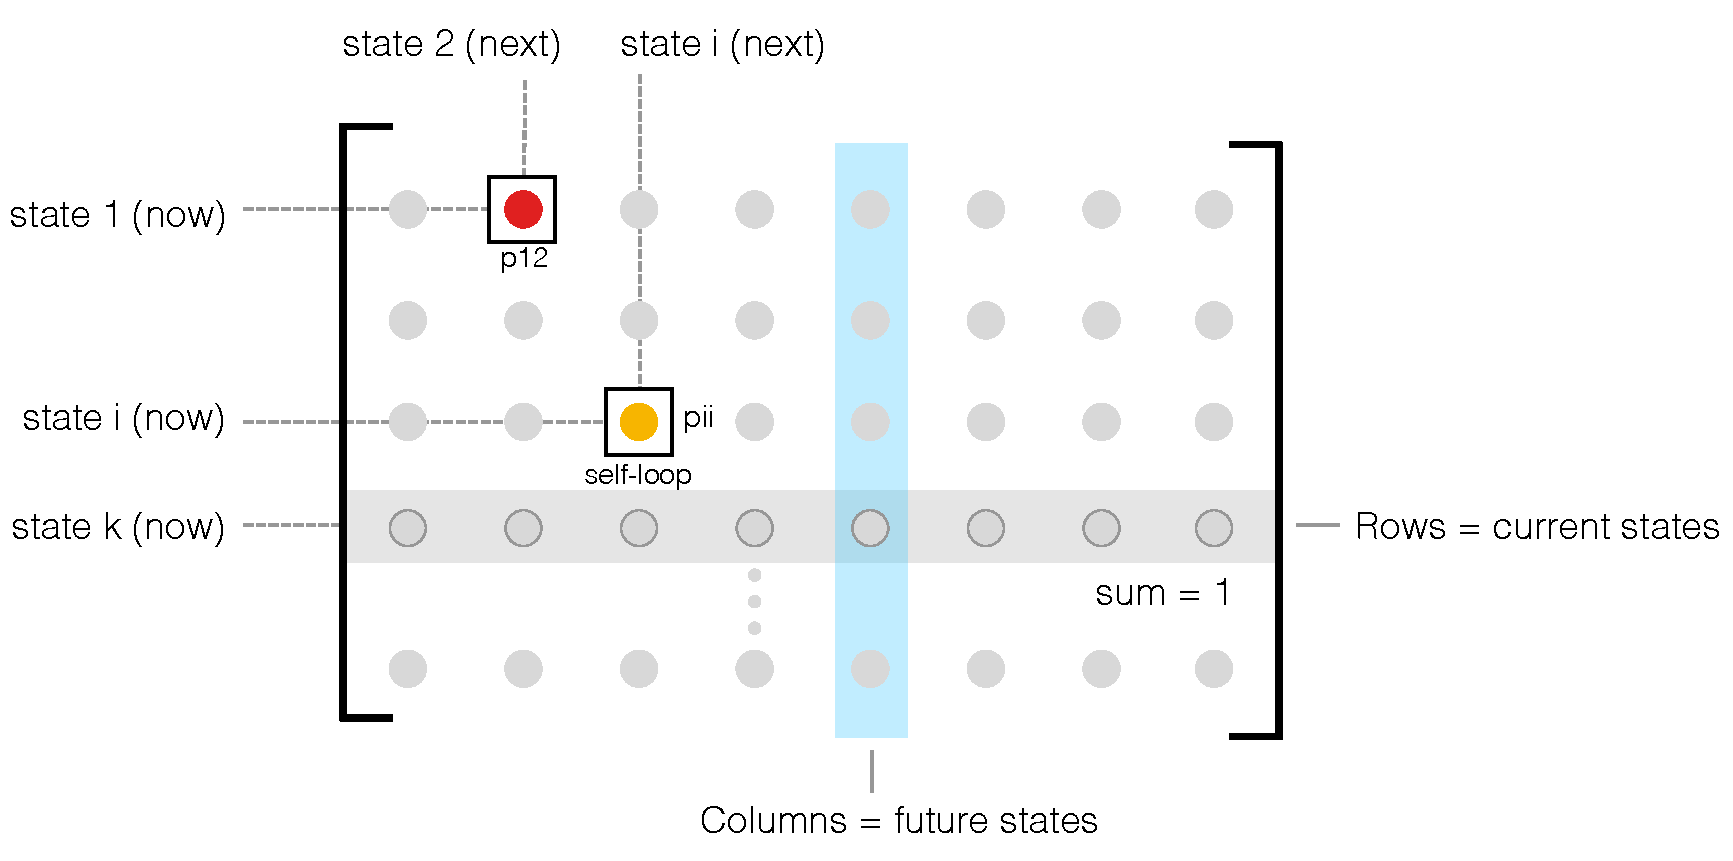
\includegraphics[width=\textwidth,height=0.64\paperheight,keepaspectratio]{assets/Fig-TransitionMatrix-Schematic.pdf}
  \lecturesource{The Transition Matrix: opening sentence and the schematic.
    Figure: ../figs/Fig-TransitionMatrix-Schematic.svg (light colors).}
\end{frame}

\begin{frame}{Properties of the Transition Matrix}
  Every transition matrix $\Pm$ has the following properties:

  \vspace{0.4em}
  \begin{itemize}\setlength{\itemsep}{0.7em}
    \item Every entry is non-negative: $p_{ij}\ge0$.
    \item Rows represent the current states, and columns represent the next
      states (our convention). Entry $p_{ij}$ is the probability of moving from
      $s_i$ to $s_j$.
    \item Every row sums to one:
      \[
        \sum_{j=1}^{N}p_{ij}=1.
      \]
      Starting from any state, the chain must move to one of the states in
      $\Sset$, including the possibility of staying where it is.
  \end{itemize}
  \lecturesource{The Transition Matrix: the three properties.}
\end{frame}

\begin{frame}{The Stationary Distribution}
  Each distribution $\pi$ is a row vector whose $j$-th element is the
  probability that the chain is in state $s_j$. The \hilite{stationary
  distribution} $\pib$ remains unchanged as the system evolves:
  \[
    \boxed{\pib=\pib\,\Pm}
  \]

  \vspace{0.2em}
  This is analogous to the steady state of a physical system. In an
  \hilite{ergodic} chain (every state can be reached from every other state,
  and the chain is not locked into a cycle), $\pib$ is the long-run fraction
  of time spent in each state.

  \vspace{0.6em}
  We estimate $\pib$ by applying the transition matrix to an initial
  distribution $\pi_0$ until the result stops changing:
  \[
    \pi_1=\pi_0\Pm,\qquad
    \pi_2=\pi_1\Pm=\pi_0\Pm^2,\qquad\ldots,\qquad
    \pi_k=\pi_{k-1}\Pm=\pi_0\Pm^k.
  \]
  \lecturesource{Algorithm: Power Iteration Method for the Stationary Distribution: definition, the steady-state analogy, and the iteration pi_k = pi_0 P^k.}
\end{frame}

\begin{frame}{Power Iteration Algorithm}
  \textbf{Initialize}: Given an ergodic transition matrix $\Pm$ with $N$ states,
  a tolerance $\epsilon>0$, and a maximum number of iterations $T$, set
  $t\gets1$, $\pi\gets[1/N,\ldots,1/N]$, and
  $\texttt{converged}\gets\texttt{false}$.

  \vspace{0.3em}
  While not $\texttt{converged}$ \textbf{do}:
  \begin{enumerate}\setlength{\itemsep}{0.2em}
    \item Compute $\pi'\gets\pi\Pm$.
    \item Check whether to stop:
      \begin{itemize}\setlength{\itemsep}{0.1em}
        \item If $\lVert\pi'-\pi\rVert_1\le\epsilon$ \textbf{then} set
          $\texttt{converged}\gets\texttt{true}$ and return $\pib\gets\pi'$.
        \item Otherwise, if $t\ge T$ \textbf{then} return $\pi'$ with
          $\texttt{converged}=\texttt{false}$ and a warning.
      \end{itemize}
    \item Update the distribution, $\pi\gets\pi'$.
    \item Increment the iteration counter, $t\gets t+1$.
  \end{enumerate}

  \vspace{0.2em}
  \textbf{Output}: the stationary distribution $\pib$, or the last estimate
  with a warning if the iteration limit was reached.
  \lecturesource{Algorithm: Power Iteration Method: Initialize, While loop, and Output. Preserve the Initialize/While/numbered-step format and the If/Otherwise branches.}
\end{frame}

\begin{frame}{Inside One Power Iteration Step}
  The update $\pi'\gets\pi\Pm$ is a left vector-matrix product: the new
  distribution is a weighted sum of the rows of $\Pm$, weighted by the current
  probabilities.

  \vspace{0.3em}
  \centering
  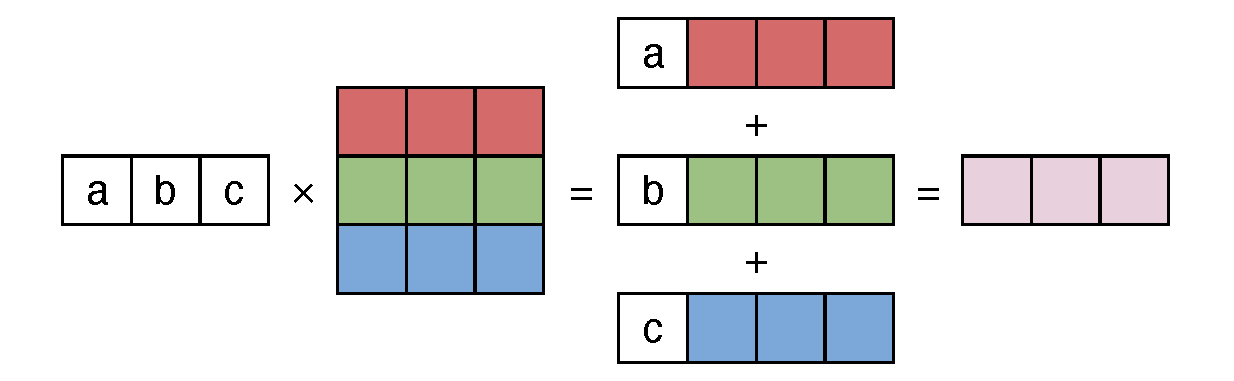
\includegraphics[width=0.78\textwidth,height=0.3\paperheight,keepaspectratio]{assets/Fig-Matrix-Vector-Left-bA-product.pdf}

  \vspace{0.3em}
  \raggedright
  \begin{itemize}\setlength{\itemsep}{0.3em}
    \item \hilite{Ergodic}: irreducible (every state can be reached from every
      other state) and aperiodic (not locked into a cycle). An ergodic chain has
      a unique stationary distribution, and power iteration converges to it from
      any start.
    \item \hilite{Spectral gap}: the difference between the largest and
      second-largest eigenvalue magnitudes of $\Pm$. Larger gaps converge faster.
  \end{itemize}
  \lecturesource{Algorithm: Power Iteration Method: the spectral gap sentence, Notes 1 and 2, and the schematic.
    Figure: ../figs/Fig-Matrix-Vector-Left-bA-product.svg (light colors).}
\end{frame}

\begin{frame}{Example: A Three-State Markov Chain}
  In this example, we explore a three-state chain whose states 1 and 3 can
  reach each other only through state 2:

  \vspace{0.2em}
  \centering
  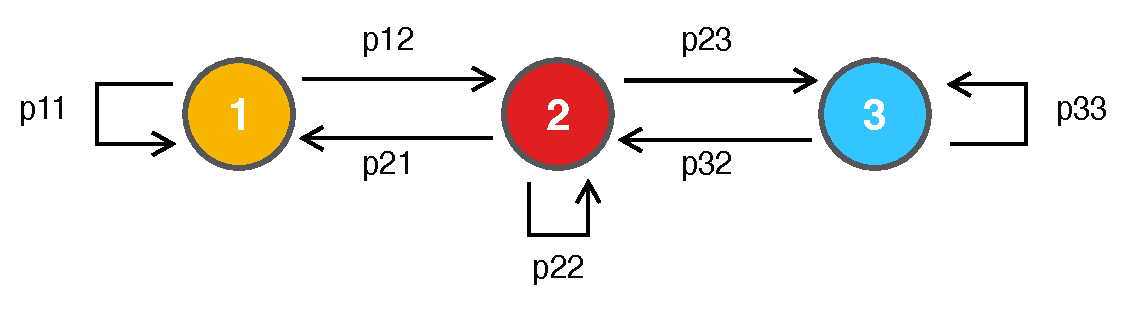
\includegraphics[width=0.8\textwidth,height=0.22\paperheight,keepaspectratio]{assets/Fig-ThreeState-MM-Schematic.pdf}

  \vspace{0.2em}
  \raggedright
  \begin{enumerate}\setlength{\itemsep}{0.3em}
    \item Build the transition matrix and check that every row sums to one.
    \item Compute the stationary distribution by power iteration, and by raising
      $\Pm$ to a large power, whose rows all approach $\pib$.
    \item Simulate the chain and compare it with independent draws from $\pib$:
      the state frequencies are similar, but the transitions differ.
  \end{enumerate}
  \slidenote{Example:}{\href{\examplelink}{Properties of Markov Models and Stationary Distributions}}
  \lecturesource{Example section. Companion example: Tasks 1--3, the three-state schematic, and the third key takeaway.}
\end{frame}

\begin{frame}{Lab: A Markov Word Generator}
  In the \href{\lablink}{lab}, we build a Markov chain whose states are the
  letters \texttt{a} to \texttt{z}:

  \vspace{0.6em}
  \begin{itemize}\setlength{\itemsep}{0.6em}
    \item we \hilite{estimate the transition matrix} from about 370,000 English
      words, counting how often each letter follows the first letter of a word,
    \item we \hilite{generate new words} one character at a time, drawing each
      character from the row of the character before it,
    \item we \hilite{check how many generated words are real}, and how that
      count changes with the length of the word.
  \end{itemize}
  \slidenote{Lab:}{\href{\lablink}{A Markov word generator}}
  \lecturesource{Lab section. Lab notebook: introduction and Learning Objectives.}
\end{frame}

\begin{frame}{Summary}
  We used Markov models to describe random systems whose future depends only
  on the present state.

  \vspace{0.5em}
  {\large\textbf{\ink{Key takeaways}}}
  \vspace{0.3em}
  \begin{itemize}\setlength{\itemsep}{0.6em}
    \item \textbf{\ink{The Markov property.}} We describe a random process with
      one-step transition probabilities instead of its entire history.
    \item \textbf{\ink{The transition matrix.}} Rows are current states and
      columns are next states; every entry is non-negative and every row sums
      to one.
    \item \textbf{\ink{The stationary distribution.}} For an ergodic chain,
      power iteration converges to the long-run fraction of time in each
      state.
  \end{itemize}

  \vspace{0.5em}
  Markov models describe random systems in applications ranging from natural
  language processing to finance and biology.
  \lecturesource{Summary: three key takeaways. The closing sentence is from the
    example's Summary.}
\end{frame}

\end{document}
